%--- 31 -------------------------------%
\item\vf{En utilisant une réplication master-slave, une lecture sur le master assurera toujours d’obtenir
les données les plus récentes}
{\vrai}
{Puisque le master est \textbf{le seul noeud accessible en écriture}, ses données sont les plus à jour (contrairement aux esclaves qui doivent être synchronisés).}


%--- 32 -------------------------------%
\item\vf{Les buckets de Riak permettent de segmenter les données en plusieurs collections d’agrégats.}
{\vrai}
{Riak est un \textbf{moteur NoSQL décentralisé/distribué} ( = Système de gestion de base de données SGBD) orienté clé-valeur. Il est très bon pour monter en charge, càd augmenter le volume de stockage, et a une haute tolérance aux pannes (peut enlever facilement un noeud en panne sans perte d'intégrité des données).
\paragraph{}
Ce SGBD stocke les clés dans des \textit{\textbf{buckets}}, qui agissent comme des \textbf{espaces de noms} pour les clés. Autrement dit deux clés peuvent porter le même nom si elles se trouvent dans des buckets différents.
\paragraph{}
Dans le modèle clé-valeur, lorsqu'on fait une requête sur une clé, toute la valeur est retournée et il n'est pas possible de cibler certaines parties (gauche fig\cite{riak-buckets}). Le système de buckets remédie d'une certaine façon à ce problème en permettant la \textbf{segmentation des données} au sein d'un même bucket (droite fig\cite{fig-riak}). Ainsi, un ensemble logique d'informations est identifé par un coupe \textit{Bucket --> Key} unique et il est possible de rechercher toutes les informations qui correspondent à une même clé.
\paragraph{}
Dans l'exemple, de la figure \cite{riak-buckets}, les données données du profil de l'utilisateur et les informations de sa session ont été séparées car il est plus intéressant de pouvoir y accéder séparemment. Chaque regroupement de donnée est alors identifé par une clé générique (elle portera le même nom dans tous les buckets, qui eux sont uniques), par exemple \textit{"sessionID\_userProfile"}. Cette clé, porteuse d'information grâce au formatage particulier de son nom, permettra ensuite d'accéder directement à un ensemble d'informations relatives à l'utilisateur, au lieu de récupérer l'ensemble de ses données.

\begin{figure}[h!]
\center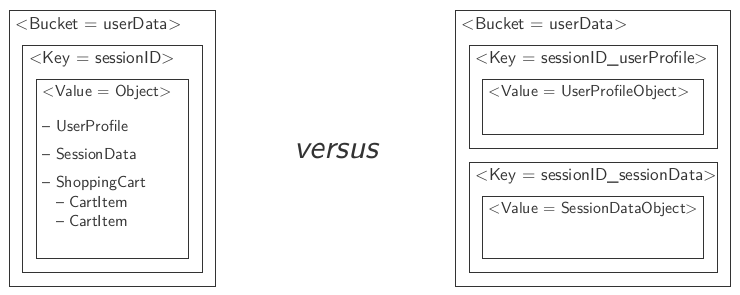
\includegraphics[scale=.3]{images/riak-bucket}
\label{riak-buckets}
\caption{Riak - système de \textit{buckets} \cite{ref1}}
\end{figure}

\paragraph{Avantages:}
\begin{itemize}
\item[$\cdot$]pratique lorsqu'on sait que les données d'une même valeur ne seront jamais utilisées en même temps -> évite de récupérer l'ensemble du contenu de la valeur
\end{itemize}
}


%--- 33 -------------------------------%
\item\vf{On ne peut pas stocker des arbres binaires comme valeurs avec Redis.}
{\faux}
{
Redis est un moteur de base de données en mémoire, utilisé pour permettre une manipulation la plus rapide possible des données. Il permet de stocker \textbf{uniquement 5 types de valeurs};
\begin{enumerate}
\item \textcolor{ltred}{\textsc{chaine de caractères, numériques ou binaires}}
\item \textcolor{ltred}{\textsc{liste (de chaines)}}: ajout/retrait à gauche ou à droite
\item \textcolor{ltred}{\textsc{ensemble de chaines non trié et sans doublons}}
\item \textcolor{ltred}{\textsc{hachage (dictionnaire) non hiérarchique}}
\item \textcolor{ltred}{\textsc{ensemble trié avec association d'une note par élément}}
\end{enumerate}
\paragraph{} 
Il n'est pas possible de créer un arbre binaire à partir d'une des structures ci-dessus.
}


%--- 34 -------------------------------%
\item\vf{Redis garantit la persistance de données.}
{\faux}
{
De base, Redis stocke les données en mémoire (cache ou virtuelle) uniquement. Une fois le serveur quitté, \textbf{toutes les données sont perdues}.
\paragraph{}
Cependant, il est de possible de configurer une sauvegarde régulière sur le disque et de la recharger.
}


%--- 35 -------------------------------%
\item\vf{Les bases de données orientée colonnes optimisent le stockage disque pour des tables qui
contiennent de nombreuses lignes.}
{\vrai}
{
Dans le modèle orienté-colonnes, différentes techniques de compressions existent pour réduire la taille de stockage des fichiers. Ces méthodes se basent sur le type de données de chaque colonne et sur le nombre de lignes qui ont une valeur est identique. Ci-dessous, trois exemples de mécanismes de compressions:
\begin{enumerate}\setlength{\itemsep}{.5em}
\item \textcolor{ltred}{\textsc{run-length encoding}}: utilisé lorsque beaucoup de données similaires sont regroupées (triées).
	\begin{figure}[h!]
	\center 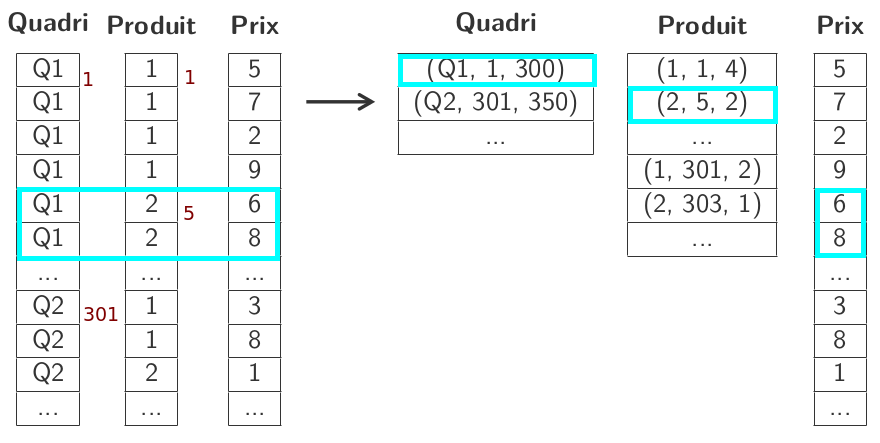
\includegraphics[scale=.35]{images/colonnes-compression-run}
	\caption{Technique de compression "\textit{Run-Length Encoding}" \cite{ref1}}\label{compression-run}
	\end{figure}
\paragraph{}
Les données identiques sont regroupées et ce sur différents niveaux. Pour éviter d'écrire sur le disque X fois la même donnée, on utilise alors un \textbf{tuple \textit{(Valeur, Adresse, Nombre)}} où l'adresse correspond à la ligne du changement de valeur. Dans l'exemple (Fig \cite{compression-run}), la valeur Q1 commence à partir de la ligne 1 et est répliquée 300 fois. En passant au niveau inférieur, on peut voit que la valeur 2 (associée à Q1) commence à la ligne 5 et est répliquées 2 fois. 
\paragraph{}
A l'étage le plus haut, il y aura donc autant de tuple qu'il y a de valeur différentes et à l'étage le plus bas, il y aura autant de valeur qu'il y a de lignes initialement.
\paragraph{}
En repartant de la colonne "Prix", on peut alors retrouver le "Produit" et le "Quadri" qui sont associés à une valeur grâce au tuples.

\item \textcolor{ltred}{\textsc{bit-vector encoding}}: utilisé lorsqu'il n'y a beacoup de lignes MAIS peu de valeurs différentes (elles ne doivent pas être triées).
	\begin{figure}[h!]
	\center 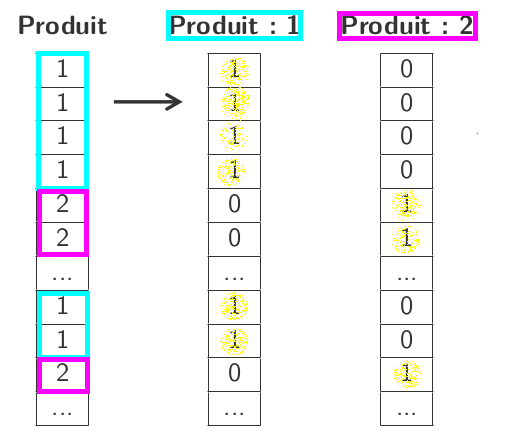
\includegraphics[scale=.35]{images/colonnes-compression-bit}
	\caption{Technique de compression "\textit{Bit-Vector Encoding}" \cite{ref1}}\label{compression-bit}
	\end{figure}
\paragraph{}
Chaque \textbf{valeur est représentée par un vecteur} dont la longeur est égale au nombre de ligne de la colonne de départ. Dans ce vecteur, on remplace la valeur associée par un 1 et les autres par 0. On ne stocke donc plus que quelques (= nombre de valeurs différentes) vecteurs de n bits pour représenter toute l'information au lieu d'un seul gros vecteur, dont la taille dépend des valeurs à encoder (sur x bits chacune).

\item \textcolor{ltred}{\textsc{dictionary encoding}}: utilisé lorsque des motifs de valeurs se répètent.
	\begin{figure}[h!]
	\center 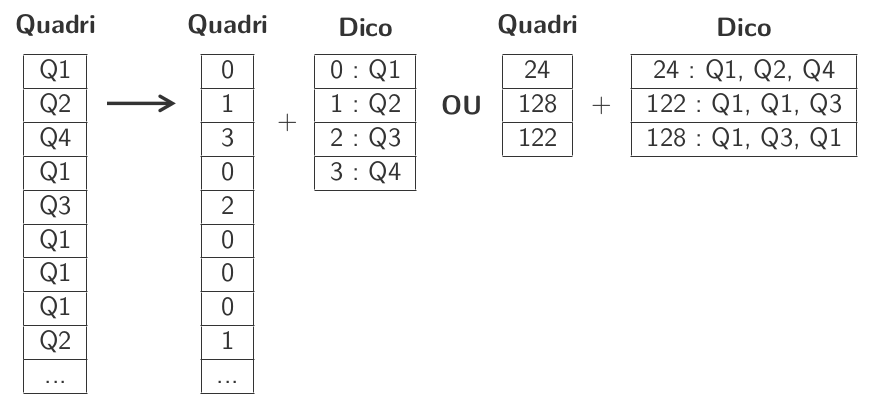
\includegraphics[scale=.35]{images/colonnes-compression-dico}
	\caption{Technique de compression "\textit{Dictionary Encoding}" \cite{ref1}}\label{compression-dico}
	\end{figure}
\paragraph{}
Deux approches sont possibles:
	\begin{itemize}
	\item[$\cdot$]on peut substituer chaque valeur par une autre qui est encodée sur moins de bits et associé la table de conversion à la nouvelle colonne (de même taille) ainsi obtenue
	\item[$\cdot$]on peut remplacer un motifs de valeurs et y associer une table ... [???]
	\end{itemize}
\end{enumerate}
}


%--- 36 -------------------------------%
\item\vf{Une base de données orientée colonnes est très adaptée lorsqu’on a plus d’opérations d’écriture
que de lecture.}
{\faux}
{Dans le modèle orienté-colonnes, les colonnes/familles de colonnes se trouvent dans des fichiers distincts. Lorsqu'on fait une lecture sur certaines colonnes, il suffit d'ouvrir les fichiers qui y correspondent. Dès lors que l'on fait une écriture pour ajouter une nouvelle entrée, il faut nécessairement ouvrir tous les fichiers... }

 
%--- 37 -------------------------------%
\item\vf{Une base de données orientée colonnes est très adaptée lorsqu’on a plus d’opérations de lecture
que d’écriture.}
{\vrai}
{}


%--- 38 -------------------------------%
\item\vf{Une base de données orientée colonnes est un map à deux niveaux.}
{\vrai}
{
Ce map à deux niveaux se compose de la façon suivante:
\begin{itemize}
\item[$\cdot$]au premier niveau -> une \textcolor{ltred}{\textsc{paire clé-valeur}} identifie une ligne
\item[$\cdot$]au second niveau -> une \textcolor{ltred}{\textsc{map de colonnes}} forme les familles
\end{itemize}
\begin{figure}[h!]
\center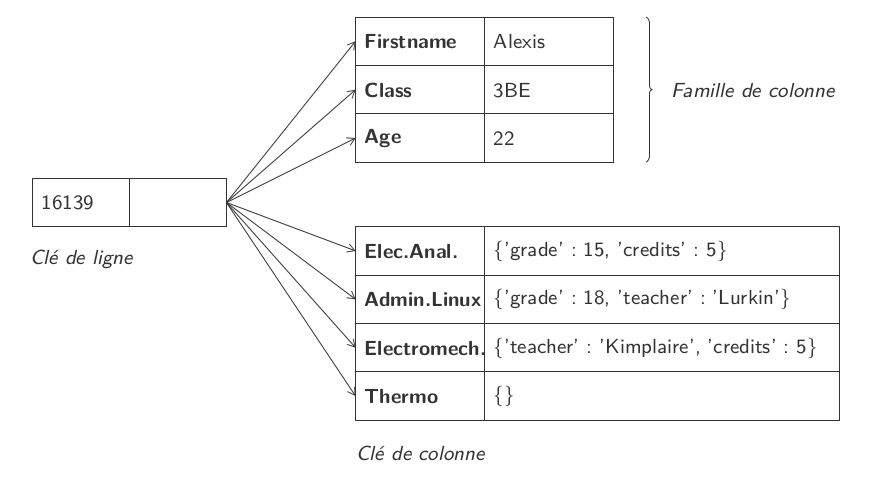
\includegraphics[scale=.3]{images/colonnes-niveaux}
\caption{Une base orientée-colonne est un \textit{map à deux niveaux} \cite{ref1}}
\end{figure}
\paragraph{}
Les colonnes qui sont "souvent accédées ensemble" sont regroupées en familles et stockées dans un même fichier. Lors de la conception d'une DB en colonnes, il est important de penser aux regroupements des colonnes car bien que l'ajout d'une colonne soit puisse se faire facilement "à chaud", des changements sur les familles sont difficilement envisageables par la suite.
\paragraph{}
Contrairemnet au modèle relationnel où toutes les colonnes d'une lignes doivent absolument être remplies (induit beaucoup de valeurs \textit{NULL}), en orienté-colonne les lignes peuvent avoir des clés colonnes différentes.
}


%--- 39 -------------------------------%
\item\vf{Dans une base de données orientée colonnes, les familles de colonnes sont de préférence définies
une fois pour toute lors de la création de la table.}
{\vrai}
{}


%--- 40 -------------------------------%
\item\vf{L’avantage de l’utilisation de colonnes plutôt que de lignes est d’offrir une vitesse d’écriture plus grande de nouveaux enregistrements.}
{\faux}
{
L'avantage du modèle colonnes est d'offrir une \textbf{vitesse de lecture plus grande}.
\paragraph{}
En effet, en relationnel classique (\textit{stockage lignes}), les lignes sont physiquement stockées les unes après les autres sur le disque. Dès lors, lorsqu'on cherche à obtenir les valeurs de certaines colonnes seulement, il faut malgré tout parcourir l'entièreté de chaque ligne. Ceci devient très contraignant, augmente considérablement le temps de lecture, lorsque le nombre de colonnes est important.
\paragraph{}
Ce problème ne se pose plus en orienté-colonne, car toutes les données d'une même colonne se trouvent dans un même fichier et sont donc physiquement contigües sur le support de stockage. La lecture des valeurs d'une (ou plusieurs) colonne(s) se fait dès lors beaucoup plus rapidement.
\begin{figure}[h!]
\center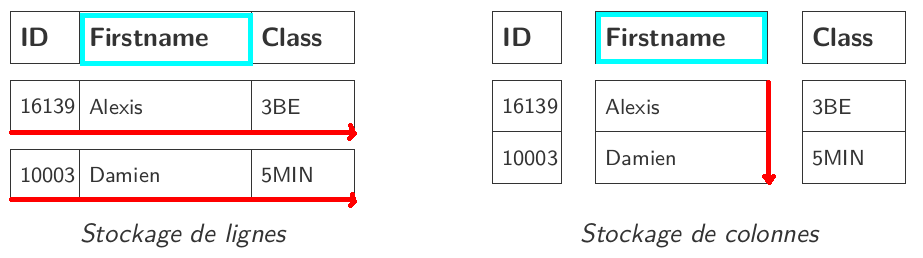
\includegraphics[scale=.35]{images/colonnes-stockage}
\caption{Modèles de stockage sur le disque \cite{ref1}}\label{colonnes-stockage}
\end{figure}
}
